\section{Learning optimal waiting time}

Our aim is to model time investment decisions in the context of perceptual decision making.
The relevant behavioral data are summarized in \cite{lak2014orbitofrontal}, figures 3 and S3.

Model 1 uses an R-learning type delta learning rule to learn a scalar waiting time ($k$) for each perceived stimulus ($\hat{x}$).
It recapitulates most aspects of the data, but fails with regard to effect of preceding outcome.
Also, it's learning rule is unstable.
I believe the way forward is to learn waiting time as a function of reward probability, and to learn reward probability from experienced stimuli.

Model 2 learns reward probability from experienced stimuli.
It learns a decision boundary, and also a sensitivity term relating the distance from boundary to reward probability.

Model 3 is incomplete, and will learn waiting time as a function of reward probability.
For simplicity, it will ignore the sensory uncertainty, and reward probability will be explicitly cued.

Model 4 will put models 2 and 3 together.

\subsection{Model 1: known boundary, one $k$ per percept}

This model learns a set of waiting times, one per stimulus, so as to maximize overall reward rate (R-learning).
It should capture dependence of waiting time on stimulus difficulty and outcome \citep[Fig 3G]{lak2014orbitofrontal} and trial history \citep[Fig S3]{lak2014orbitofrontal}.

\subsubsection{Model description}

Stimulus is represented by $x \in X = \{5, 30, 45, 55, 70, 95 \}$, and the corresponding stimulus category $c \in \{0,1\} = H(x-50)$, where $H(z)$ is the Heaviside function
\begin{equation}
H(z) =
\begin{cases}
1 & \text{if }  z > 0 \\
0 & \text{if }  z < 0 \\
\end{cases}
\label{eq:heavi}
\nonumber
\end{equation}

The subject does not know the stimulus $x$, but the percept $\hat{x}$ defined as
\begin{equation}
    \hat{x} = \underset{x' \in X}{\operatorname{argmin}} \left( x' - x + \epsilon \right)
    \nonumber
\end{equation}
where $\epsilon$ is a Gaussian noise term.
That is to say, the\textbf{ percept is a noise corrupted stimulus rounded to the nearest element in the original stimulus set}.

On each trial, the subject makes two decisions:
\begin{enumerate}
    \item a perceptual decision $a = H(\hat{x} - 50)$ (ie. known boundary, no decision noise)
    \item a time investment (TI) decision $ k_{\hat{x}} \in \mathbb{R}_+ $
\end{enumerate}

A reward is earned whenever the perceptual choice $a$ is correct and waiting time ($k_{\hat{x}}$) is longer than reward delay $d$ ($d \sim Exp(1.5), d \in \left[0.5,8\right]$).

%\subsubsection{Learning $k_{\hat{x}}$}

The subject learns one TI value $k_{\hat{x}}$ per percept $\hat{x}$, and $k_{\hat{x}}$ is learned according to a delta learning rule that maximizes overall reward rate.

Reward rate $\rho$ is learned from experience as in \cite{constantino2015learning}.
For reward $r=1$ for rewarded trials and $0$ otherwise, and trial duration $\tau$, the learning target $\delta$ is defined as follows:
\begin{align}
\tau &=
\begin{cases}
d & \text{if trial rewarded} \\
k_{\hat{x}} & \text{if not rewarded}\\
\end{cases}\\
\delta &= r - \tau \rho
\nonumber
\end{align}

The actual updating equations are
\begin{align}
    k_{\hat{x}} &\leftarrow k_{\hat{x}} + \eta_k \delta \\
    \rho &\leftarrow \rho + (1-(1-\eta_\rho)^\tau) \delta
\end{align}
where $\eta_k, \eta_\rho \in [0,1]$ are learning rate parameters.

\subsubsection{Simulation}

This model captures several aspects of \cite{lak2014orbitofrontal}.
The psychometric looks reasonable, and waiting time depends on stimulus difficulty and whether choice was correct or incorrect (figure \ref{fig:mod1f3}).
As in figure S3 of \cite{lak2014orbitofrontal}, performance is the same irrespective of whether previous trial was correct or incorrect, or whether waiting time on previous trial was above or below median (long vs short) (figure \ref{fig:mod1fs3}).
Furthermore, waiting time is higher when previous trial was a long one.

Points where this model fails:
\begin{itemize}
    \item Waiting time does not depend on outcome of previous trial (figure \ref{fig:mod1fs3}, top right). \textbf{Fix}: make waiting time $k$ a function of reward probability (model 2); learn reward probability from experience (models 3-4); learn decision boundary.
    \item Target reward rate is not a fixed point; degrades after initial improvement (fig \ref{fig:mod1f3}, bottom right). \textbf{Fix}: Delta learning rule is intuitively ok, but defective; use a principled one (see below).
\end{itemize}

\begin{figure}[t!]
    \centering
    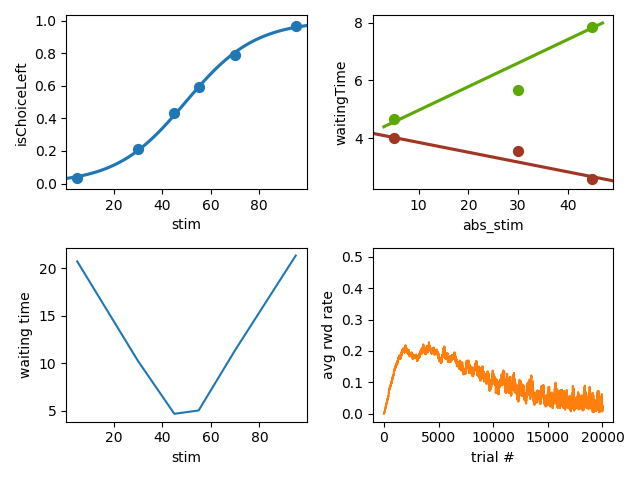
\includegraphics[width=.6\linewidth]{dual2afc/myplot.png}
    \caption{Model 1.\\
    (\textbf{top left}) Psychometric curve. \\
    (\textbf{top right}) Waiting time dependence on stimulus difficulty and outcome (green: correct, red: incorrect). \\
    (\textbf{bottom left}) Final values of $ k_\hat{x} $. \\
    (\textbf{bottom right}) Evolution of average reward rate $\rho$ through learning.}
    \label{fig:mod1f3}
\end{figure}

\begin{figure}[h!]
    \centering
    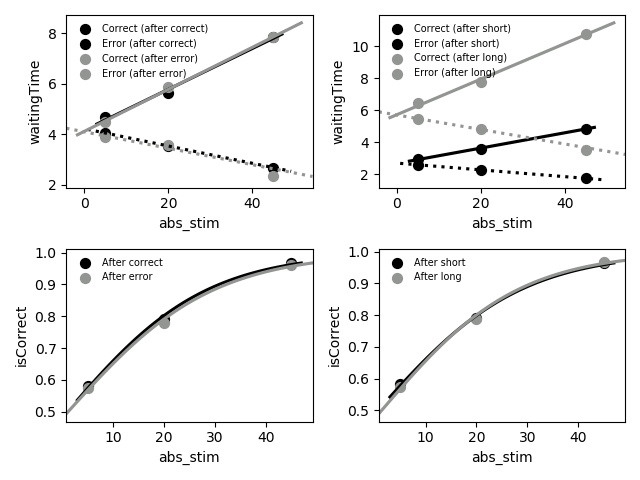
\includegraphics[width=.6\linewidth]{dual2afc/myplot2.png}
    \caption{Model 1. Plots analogous to figure S3 in \cite{lak2014orbitofrontal}}
    \label{fig:mod1fs3}
\end{figure}

%\subsection{Task description}

%\subsection{Learning the decision boundary $\hat{b}$}
%\clearpage
\subsection{Model 2: learning reward probability from experienced perceptual decisions}

\subsubsection{Model description}

Let stimulus be represented by $x \in \mathbb{R}$, and the corresponding stimulus category $c \in \{0,1\} = H(x-b)$, where $b$ is an unknown category boundary and $H(z)$ is the Heaviside function.

Let the percept be $\hat{x} = x + \epsilon$, where $\epsilon$ is a Gaussian noise term.
The subject must on every trial make a choice $a \in \{0,1\}$ based on $\hat{x}$.
Assuming no catch trials, a trial is rewarded whenever choice $a$ matches stimulus category $c$.
Thus, in order to maximize rewards subjects must be able to estimate category $c$ from knowledge of $\hat{x}$.

Just as in a logistic regression \cite[Section 4.3.2]{bishop2006pattern}, the posterior probability of stimulus category $c$ can be written as a logistic sigmoid $g(z)$ acting on a linear function of the percept $\hat{x}$:
\begin{align}
g(z) &= \frac{1}{1+\exp(-z)} \\
P(c = 1 \mid \hat{x}) &= g(m(\hat{x}-\hat{b})) \label{eq:Pcgperc} \\
P(c = 0 \mid \hat{x}) &= 1 - g(m(\hat{x}-\hat{b}))
\end{align}
with $m, \hat{b} \in \mathbb{R}^+$.
%Thus, a greedy decision rule can be defined as $a = H(\hat{x}-\hat{b})$, where the decision boundary $\hat{b}$ must be learned to approximate the true category boundary $b$.

For a data set with $N$ trials, the likelihood of observed stimulus category as a function of parameters  $m, \hat{b}$ can be written as 
\begin{equation}
    P(\mathbf{c} \mid m, \hat{b}) = \prod_{n=1}^N g(m(\hat{x}_n-\hat{b}))^{c_n} \left(1-g(m(\hat{x}_n-\hat{b}))\right)^{(1-c_n)}
\end{equation}

Parameters can then be learned by minimizing the negative log likelihood
\begin{equation}
    L = - \sum_{n=1}^N
    {c_n} \log g(m(\hat{x}_n-\hat{b})) + 
    {(1-c_n)} \log \left(1-g(m(\hat{x}_n-\hat{b}))\right)
\end{equation}

A subject performing the task could minimize $L$ on the flight by stochastic gradient descent, that is, by computing on each trial the gradient $ \nabla L = \left[\frac{\partial L}{\partial m}, \frac{\partial L}{\partial \hat{b}} \right]^T $ and using it to update its parameter estimates.

Specifically, for trial $n$ and $z_n = m(\hat{x}_n-\hat{b})$, it is useful to establish
\begin{align}
     \frac{\partial L}{\partial z_n} &= \frac{\partial}{\partial z_n}\left[ -{c_n} \log g(z_n) -
    {(1-c_n)} \log \left(1-g(z_n)\right) \right] \nonumber \\
    %        &=  (-c_n) g(z_n)^{-1} g(z_n) \left(1-g(z_n)\right) \nonumber  \\
    %        &- (1-c_n) (-1)  \left(1-g(z_n)\right)^{-1} g(z_n) \left(1-g(z_n)\right) \nonumber \\
    %        &=  (-c_n) \left(1-g(z_n)\right) + (1-c_n) g(z_n)   \nonumber \\
    %        &=  (-c_n) + c_n g(z_n) + g(z_n) -c_n g(z_n)   \nonumber \\
    &=   g(z_n) -c_n   \label{eq:dLdz} \\
    \frac{\partial z_n}{\partial \hat{b}} &= -m \\
    \frac{\partial z_n}{\partial m} &= \hat{x} - 
    \hat{b}
\end{align}

from what it follows by the chain rule that

\begin{align}
    \nabla L &=
    \begin{bmatrix}
    (\hat{x}-\hat{b}) (g(z_n) - c_n)   \\
    m (c_n - g(z_n))
    \end{bmatrix}
\end{align}

Parameter updating would then proceed according to
\begin{align}
    m_{n+1} &= m_{n} - \eta (\hat{x}-\hat{b}) (g(z_n) - c_n) \\
    \hat{b}_{n+1} &= \hat{b}_{n} - \eta m (c_n - g(z_n)) \label{eq:update_b}
\end{align}
where $\eta$ is a step size (learning rate) parameter.

\subsubsection{Simulation}
With parameters $\hat{b}, m$ initialized to $0$, the model was run for $10^5$ trials with different levels of sensory noise $\epsilon$.
Decision boundary quickly converged to its true value $0.5$, and oscillated around it throughout learning.
The slope parameter $m$ consistently converged, albeit to different values depending on levels of sensory noise (figure \ref{fig:mod3}, left column).

\begin{figure}[h!]
    \centering
    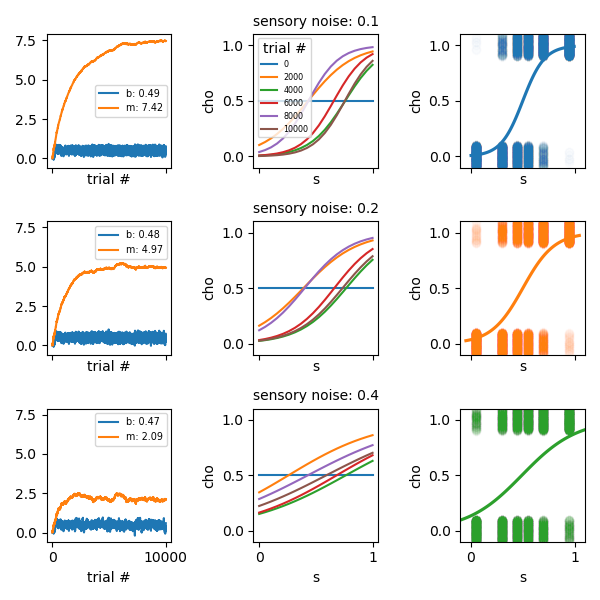
\includegraphics[width=.8\linewidth]{dual2afc/myplot3.png}
    \caption{Model 2, at different levels of sensory noise (rows). \\
    (left) Learning of decision boundary $\hat{b}$ and slope $m$ is stable. \\
    (center) Learned sigmoid at different stages of learning. \\
    (right) Psychometric curve at the end of learning.}
    \label{fig:mod3}
\end{figure}

An agent whose only concern is to get the perceptual decision right (ie. no time investment decision), has only to learn the decision boundary $\hat{b}$, and could thus set $m$ to any constant value in $\mathbb{R}_+$, say $m=1$ for convenience.
%The learning equation \ref{eq:update_b} could then drop the $m$ term, and could probably be expressed in terms of reward rather than category $c$.
Notice that the magnitude of the update of $\hat{b}$ (equation \ref{eq:update_b}) still depends on the distance between percept and boundary (since  $z_n = m(\hat{x}_n-\hat{b})$).

However, if the agent is also learning a time investment decision, it will probably be required to estimate $P(c \mid \hat{x})$ (equation \ref{eq:Pcgperc}), which depends on $m$.
In fact, psychometric curves observed under different noise levels were captured by different values of $m$  (figure \ref{fig:mod3}).
%given that $H(g(m(\hat{x}-\hat{b})))$ does not depend on $m$,

\subsection{Model 3: time investment as function of reward probability, isolated from perceptual decision}

An animal should wait at the reward port whenever he believes a reward is coming, and abort the trial otherwise.
This decision should be based on a model similar to \cite{starkweather2017dopamine}, where belief about whether a reward is available should be informed by both perceptual confidence and elapsed time at the reward port.

These components can be isolated, eg. on a different task in which pre-reward delays have the same distribution but reward probability is explicitly cued.

Roughly, this will rely on a Bayesian procedure estimating posterior probability of reward given time waited with no reward delivered, where the prior is the cued reward probability, and the likelihood is the CDF of the reward delay distribution.
Any quantity of time waited during which no reward is delivered is evidence that choice was incorrect.
The threshold to abort a trial might be learned so as to maximize average reward rate.

I have relevant code for this that I wrote when analyzing waiting time data in matching task, but haven't yet had the time to put it here. 
%\clearpage
\subsection{Model 4: learning both reward probability and time investment decisions}

Models 2 and 3 plugged together.
Should give our final result.

\clearpage
\begin{align}
\text{Return } G &= P(\text{reward} \mid \text{choice} , \text{waiting time } k) - \text{opportunity cost} \nonumber
\\
\text{opportunity cost } &=  k \times   \text{average reward rate } \rho \nonumber
\\
\frac{\partial G}{\partial k} \nonumber &= 0 \\
k &= -\beta \log \frac{\beta \rho}{P(\text{reward})} \nonumber \\
\text{for } \beta = 1 \qquad k &= \log \frac{P(\text{reward})}{\rho} \nonumber
\end{align}

\clearpage

optimal waiting time $k = \log \frac{P(\text{reward})}{\rho} $